\chapter{\label{chap:scripttests}Executing Script Driven Tests}

The tests described in this chapter are designed to exercise all accessible objects in the core
GMAT engine, in as many combinations as is feasible.  This object coverage is performed by running
GMAT scripts designed to interact with the accessible objects from the Graphical User Interface.
Each script produces output.  The system testers examine this output, and, when possible, compare it
with the configuration managed output produced from previous runs of the scripts.  The procedure
followed when running scripted tests is documented in the sections of this chapter.

\begin{figure}[htb]
\begin{center}
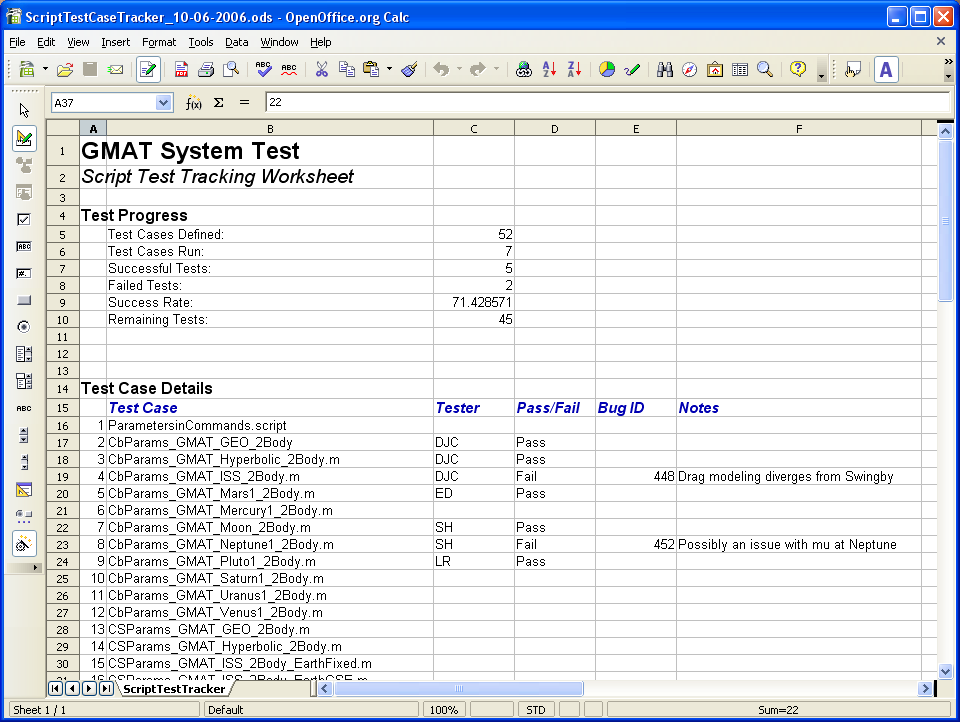
\includegraphics[460,346]{Images/TestTrackingWorksheet.png}
\caption{\label{figure:ScriptTestTracker2}The Script Test Tracking Spreadsheet}
\end{center}
\end{figure}

\section{Script Test Case Management}

The System test cases are managed from a spreadsheet generated at the conclusion of the system test
preparation process.  Figure~\ref{figure:ScriptTestTracker2} shows an example of this test
tracking spreadsheet for the script based tests\footnote{The test tracking spreadsheets, unlike the traceability matrix spreadsheet, can be saved in either OpenOffice or Excel format.}, as it looks
partway through a test cycle.

The test procedure for script based tests is relatively straightforward.  Testers follow these steps when executing the system tests:

\begin{enumerate}
\item Obtain the latest versions of the scripts and known good results from the system test repository.
\item Identify the tests each tester needs to run.
\item Open GMAT\footnote{GMAT should only be opened one time for any given testing period.  All tests run during that test period -- typically a morning or afternoon -- should be run in the same instance of GMAT.  This helps ensure that the system is stable over long periods of time.  If the system is shut down, either by the user or through a system crash, that event should be noted.}.
\item Run each test following the procedure in \ref{section:RunningScriptTests}.
\item As each test is run, record the summary results in a local copy of the test tracking
spreadsheet.
\item When anomalies are found in testing, record them local test case report files.
\item At the end of each day or when testing is finished, whichever occurs first, gather the test
case reports generated from the tests and place them in the folder used to gather the test results.
\item Close GMAT at the end of the test period.
\item At the end of each day or when testing is finished, whichever occurs first, save the local
test tracking spreadsheet with the name <spreadsheetName>\_<tester's initials> in the folder
used to gather the test results.
\item Upon completion of all assigned test cases, report that status to the system test lead.
\end{enumerate}

\section{\label{section:RunningScriptTests}Running the Scripted System Tests}

By their very nature, the GUI based tests described in Chapter~\ref{chap:guitests} follow a relatively unstructured execution sequence that mandates more structured test case documents to ensure complete system testing.  In contrast, the script based tests follow a linear execution sequence once the scripts have been written and debugged.  The rest of this chapter describes the procedure followed for the scripted tests.

\subsection{Procedure}

Each scripted test case has an associated, configuration managed script.  Most script test cases also have output data files used to compare the obtained script outputs with validated GMAT output files.  A tester follows this procedure to perform the associated system test:

\begin{enumerate}
\item Open a blank test case report file\footnote{The test case report file is only needed for
script based tests is an anomaly is found during testing.  In practice, the test case report only
needs to be opened when an anomaly is found.}.
\item Open the script in GMAT.
\item\label{item:repeatStart} Compare the resources displayed in GMAT with the resources defined in the script. Enter any anomalies in the test case report.
\item Compare the mission sequence in the script with the mission sequence displayed in GMAT.
Enter any anomalies in the test case report.
\item Run the script.
\item Examine each plot and 3D view that opens.  Enter any anomalies on the in the test case report.
\item Compare the output results from the run with the known good data.  Enter any anomalies in the test case report.
\item Press the run button.
\item Examine each plot and 3D view that opens.  Enter any anomalies on the in the test case report.
\item Compare the output results from the run with the known good data.  Enter any anomalies in the test case report.
\item\label{item:repeatEnd} Open the script in the editor window, and press the ``Build and Run''
button.
\item Examine each plot and 3D view that opens.  Enter any anomalies on the in the test case report.
\item Compare the output results from the run with the known good data.  Enter any anomalies in the test case report.
\item Save the script to a new file with the name Saved\_<Test case name>.
\item Load the saved script into GMAT.
\item Repeat steps~\ref{item:repeatStart} through~\ref{item:repeatEnd}
\item If any anomalies have been found, fill in the header and summary data on the test case
report, and save it with the file name ``<test case>\_YYYYMMDD.report'', where YYYYMMDD indicate
the year, month and day the test was run.
\end{enumerate}

\subsection{A Note on Run Frequency}

The script based tests can be run much more frequently than is feasible for the GUI tests.  Scripts that are identified as being run more frequently than at the system test frequency follow a somewhat abbreviated procedure from that defined at the system test level.  The purpose of the more frequent testing is to help catch errors in the system prior to format system testing.  Teh abbreviated test procedure performed for each weekly or monthly test is presented here:

\begin{enumerate}
\item Open the script in GMAT.
\item Run the script.
\item Examine each plot and 3D view that opens.  Report any anomalies.
\item Compare the output results from the run with the known good data.  Report any anomalies.
\item If any anomalies have been found, enter a new anomaly in the bug tracking system.
\end{enumerate}

These tests follow the full system test procedure when run as part of the system test suite.

\subsection{Reporting Results}

At the start of the system test process, a central location was established for collection of the
test results.  The final step performed by the system testers is to copy their test case worksheets and local test tracking worksheet to this central location.  This action is performed each day the
system tests are run so that the progress of the system test execution can be evaluated.  Upon
completion of all system testing by a specific tester, a final update is made and the system test
lead is notified that that tester has completed the assigned tests.  Chapter~\ref{chap:reporting}
describes the consolidation of the collected test results into a system test report.
